% Chapter 1

\chapter{Introducción general} % Main chapter title
En este capítulo se hace una breve introducción a la necesidad que condujo al desarrollo del trabajo. Se presenta el concepto de internet de las cosas o IoT (del inglés \textit{Internet of Things}) y el estado del arte de dispositivos similares. Asimismo, se explica el objetivo y los alcances del trabajo.
\label{Chapter1} % For referencing the chapter elsewhere, use \ref{Chapter1} 
\label{IntroGeneral}

%----------------------------------------------------------------------------------------

% Define some commands to keep the formatting separated from the content 
\newcommand{\keyword}[1]{\textbf{#1}}
\newcommand{\tabhead}[1]{\textbf{#1}}
\newcommand{\code}[1]{\texttt{#1}}
\newcommand{\file}[1]{\texttt{\bfseries#1}}
\newcommand{\option}[1]{\texttt{\itshape#1}}
\newcommand{\grados}{$^{\circ}$}

%----------------------------------------------------------------------------------------

%\section{Introducción}

%----------------------------------------------------------------------------------------
\section{Internet de las cosas en la agricultura}
En los últimos años la agricultura ha enfrentado muchos desafíos, desde una creciente población mundial a ser alimentada, hasta requisitos de sostenibilidad y restricciones ambientales debido al cambio climático y el calentamiento global.

La agricultura es uno de los sectores que más sufre la escasez de agua que existe actualmente en el mundo, uno de los objetivos de implementar la tecnología IoT en este sector, es el de lograr una gestión eficiente y sostenible de los recursos hídricos.

Esto obliga a implementar soluciones que permitan modernizar las prácticas agrícolas. En este contexto, la Agricultura 4.0 representa la última evolución de la  agricultura de precisión. La misma se encuentra basada en el concepto de agricultura inteligente, donde convergen el uso de internet de las cosas, computación
en la nube, aprendizaje automático para el análisis de grandes volúmenes de datos, vehículos no tripulados y robótica \citep{Agriculture4.0}.

\subsection{Internet de las cosas}
El concepto de internet de las cosas se refiere a la interconexión digital de dispositivos y objetos a través de una red, es decir, dispositivos como sensores y/o actuadores, equipados con una interfaz de comunicación, unidades de procesamiento y almacenamiento. Estos dispositivos tienen la capacidad de adquirir, intercambiar y transferir datos a la red mediante alguna tecnología de comunicación inalámbrica \citep{WirelessComunications}.

El IoT puede usarse a favor de la sostenibilidad, no cabe duda de que Internet es un facilitador de iniciativas sostenibles. De acuerdo con el Foro Económico Mundial la mayoría de los proyectos con internet de las cosas se centran en la eficiencia energética en las ciudades, energías sostenibles y el consumo responsable \citep{InternetDeLasCosas}. 
\\Por ejemplo:
\begin{itemize}
  \item Eficiencia energética: en este sector se interconectan sensores, algoritmos y redes de comunicación para anticipar la demanda eléctrica y así realizar una distribución sostenible de la energía para reducir el precio del kW.
  \item Uso del agua: esta tecnología pone en funcionamiento máquinas para recoger datos en tiempo real que permitan hacer uso eficiente del agua y reducir su consumo.
  
\end{itemize}

\subsection{Sistemas de monitoreo de cultivos agrícolas}
Los sistemas de monitoreo de cultivos agrícolas se encargan de monitorear
las distintas variables ambientales a las que están expuestos los cultivos agrícolas, los datos adquiridos ayudan a la toma de decisiones y a manejar de una manera eficiente los recursos con los que cuentan los agricultores.

Cuentan con tres partes fundamentales: 
\begin{itemize}
  \item El nodo sensor, que en sí sería la parte física o hardware, es generalmente de bajo consumo.
  \item El firmware que abarca la lógica del sistema y se encarga de realizar la adquisición, procesamiento y transferencia de datos que puede o no estar sobre un sistema operativo de tiempo real.
  \item Nube o plataforma IoT, que ofrecen diferentes servicios como ser almacenamiento, procesamiento, análisis, visualización, etc. Esta parte del sistema permite al usuario del sistema poder visualizar los valores de las variables medidas y así poder tomar decisiones con respecto a las mediciones.
\end{itemize}
%----------------------------------------------------------------------------------------

\section{Estado del arte}

Durante la etapa de investigación del trabajo se realizó la búsqueda de productos comerciales en el mercado local e internacional.
Se encontraron algunos productos de similares características al que se pretende realizar, un dato interesante a resaltar es que todos los productos encontrados son del mercado internacional, no se encontró ningún producto o empresa que ofrezca este tipo de soluciones
en el mercado local.

A continuación se describen los productos encontrados, estas opciones varían con respecto a la tecnología que utilizan.

\subsection{Libelium}

Smart Agriculture PRO figura \ref{fig:Modulo-libelium} es un módulo de IoT que está diseñado para realizar monitoreo de viñedos para mejorar la calidad del vino, riego selectivo en campos de golf y control de condiciones en invernaderos, entre otros.
Permite monitorear múltiples parámetros ambientales que involucran una amplia gama de aplicaciones, desde el análisis del desarrollo en crecimiento hasta la observación del clima. Para ello se ha dotado de sensores de temperatura y humedad del aire y del suelo, luminosidad, radiación solar, velocidad y dirección del viento, precipitaciones, presión atmosférica, humedad de las hojas, distancia y diámetro del fruto o tronco \citep{ModuloAgriculture}.
\vspace{1cm}

\begin{figure}[htbp]
	\centering
	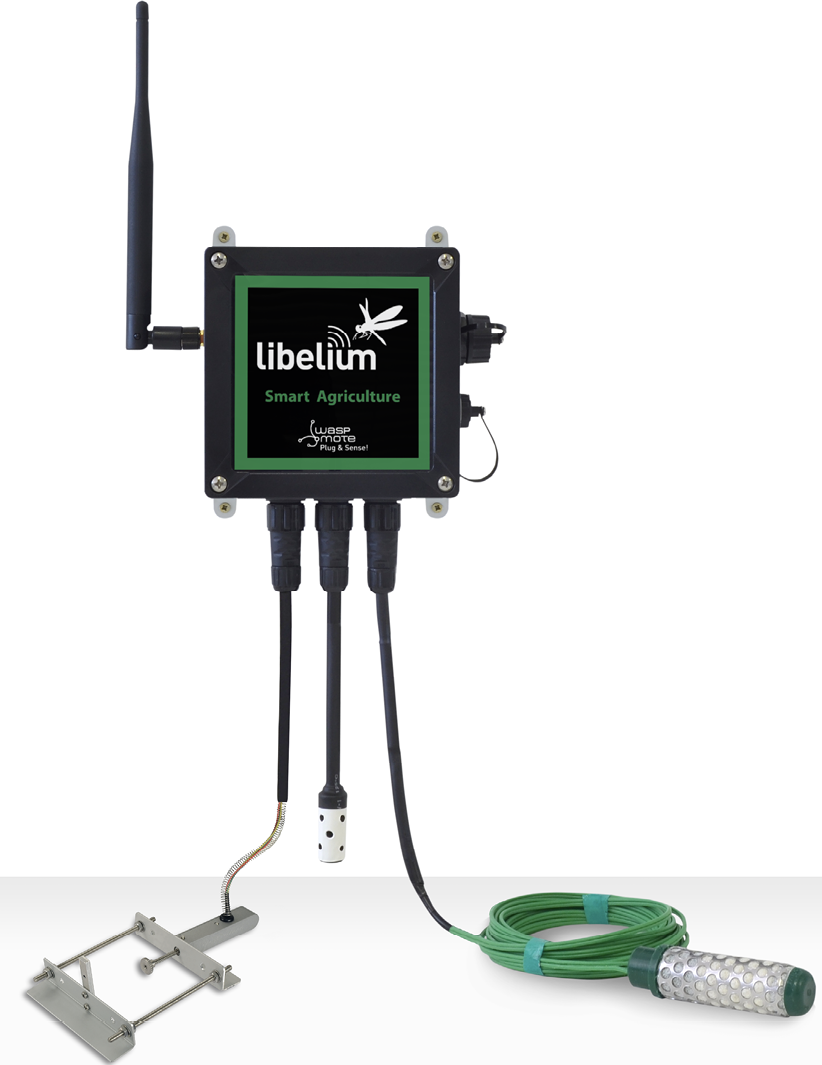
\includegraphics[width=5cm, height=6cm]{./Figures/modulo_libelium.png}
	\caption{Módulo Smart Agriculture PRO.}
	\label{fig:Modulo-libelium}
\end{figure}
\vspace{1cm}

\subsection{Nodo RF-M1 DropControl}

El nodo RF-M1 es adecuado para tareas de monitoreo simples como parte de una red DropControl o por sí solo. Posee una combinación de entradas que le permite realizar múltiples tareas de monitoreo y almacenarlas en la nube. En la figura \ref{fig:Modulo-Dropcontrol} se muestra el módulo físicamente \citep{ModuloAgricultureDos}.
Características del dispositivo: 
\begin{itemize}
  \item Redes RF \textit{mesh} o comunicación celular.
  \item Energía autónoma, solar + batería.
  \item Actualización del firmware vía aérea, configuraciones y soporte por internet.
  \item Protección externa IP65.
  \item Amplia variedad de compatibilidad con sensores.
  \item Unidad de bajo costo para resolver necesidades básicas de monitoreo. 
\end{itemize}

\begin{figure}[htbp]
	\centering
	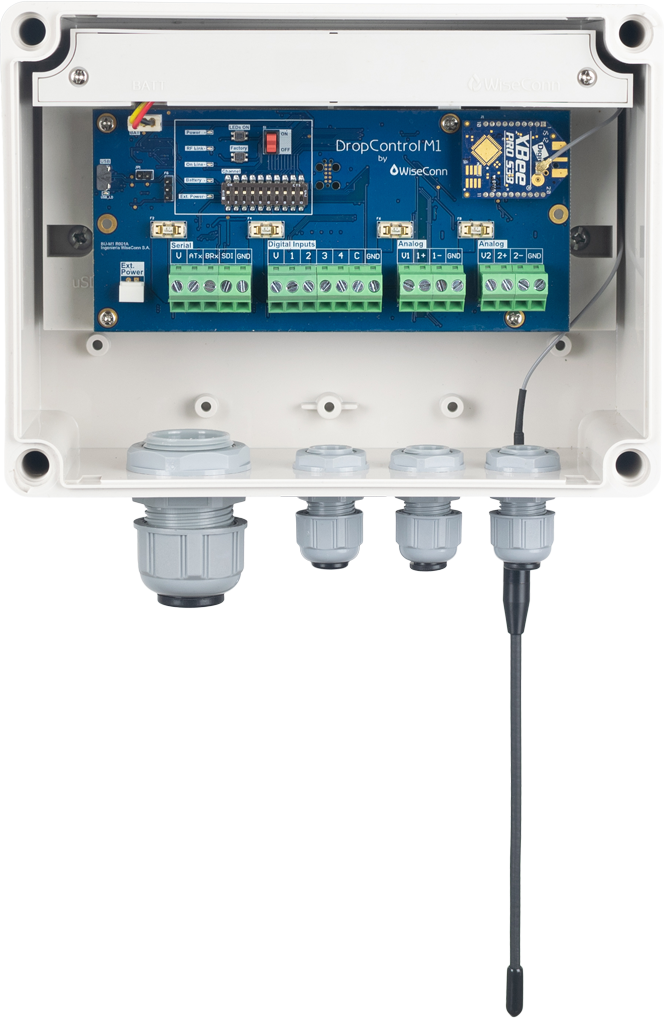
\includegraphics[width=6cm, height=7.5cm]{./Figures/modulo_dropcontrol.png}
	\caption{Módulo RF-M1 de DropControl.}
	\label{fig:Modulo-Dropcontrol}
\end{figure}
%----------------------------------------------------------------------------------------

\section{Objetivo y alcances}

\subsection{Objetivo}
El objetivo principal del trabajo es el diseño e implementación de un prototipo funcional de un sistema de monitoreo de cultivos agrícolas.
\subsection{Alcances}

\begin{itemize}
  \item Implementación de un prototipo funcional con hardware de bajo consumo. 	
  \item Desarrollo del firmware sobre un sistema operativo de tiempo real.
  \item Transmisión de la información por red celular.
  \item Visualización de los datos en ThingsBoard \citep{THINGSBOARD}.
\end{itemize}